\documentclass[pdflatex,sn-mathphys-num,iicol]{sn-jnl}

\usepackage[T1]{fontenc}
\usepackage{amsmath,amssymb}
\usepackage{float}
\floatstyle{ruled}
\newfloat{algorithm}{tbp}{loa}
\floatname{algorithm}{Algorithm}
\usepackage{algpseudocode}
\usepackage{booktabs}
\usepackage{graphicx}
\usepackage{tabularx}
\usepackage{tikz}
\usepackage{pgfplots}
\pgfplotsset{compat=1.17}
\usepgfplotslibrary{groupplots}
\usetikzlibrary{arrows.meta,calc,positioning}
\hypersetup{hypertexnames=false}
\newcommand{\checkpointsha}{\texttt{c6f98247\allowbreak{}e7c731a5\allowbreak{}67aaf37c\allowbreak{}a7b808be\allowbreak{}ff588b68\allowbreak{}7623e028\allowbreak{}b25a2e1d\allowbreak{}846e96e7}}

\raggedbottom
\setcounter{dbltopnumber}{2}

\begin{document}

\title[AC-MOT]{AC-MOT: Optimization-Guided Adaptive Detector Operating-Point Control for Aerial Multi-Object Tracking}

\author*[1]{\fnm{Ahmed Gouda} \sur{Ismail}}\email{a7medgouda1@gmail.com}
\author[1]{\fnm{Mohamed S.} \sur{Mohamed}}\email{mohamedms@mtc.edu.eg}
\author[2]{\fnm{Tarek Ahmed} \sur{Mahmoud}}\email{tarek.mohamed@eui.edu.eg}

\affil*[1]{\orgdiv{Computer Engineering and Artificial Intelligence Department}, \orgname{Military Technical College}, \orgaddress{\city{Cairo}, \country{Egypt}}}
\affil[2]{\orgdiv{Computer Engineering Department}, \orgname{Egypt University of Informatics}, \orgaddress{\city{Cairo}, \country{Egypt}}}

\abstract{Scenes recorded by unmanned aerial vehicles change over time in object density, object size, illumination, and blur. Most tracking-by-detection pipelines still run the detector at one fixed operating point. AC-MOT is a training-free control layer that treats the detector operating point as part of the multi-object tracking (MOT) system. It uses only the current frame and past tracker output. At run time it reads inexpensive scene cues and selects the detector confidence threshold, the non-maximum-suppression (NMS) IoU threshold, and the input resolution. The detector and the tracker are not retrained or modified. The controller was developed through optimization: a quality-oriented Optuna profile, an identity-aware MOTA/IDS Pareto study, transfer and cross-pipeline studies, and a modern controller developed with sequence-level cross-validation on separate calibration sequences and then frozen. On a frozen evaluation of seven VisDrone2019-MOT sequences with a YOLO11m detector, AC-MOT raises HOTA by 2.937 points with ByteTrack (95\% CI [2.356, 3.375]) and by 1.325 points with the recent OATrack tracker (95\% CI [0.200, 2.264]); MOTA rises by 17.995 and 6.318 points. On a Tesla T4 GPU, the controller adds only 4.26 ms per frame with ByteTrack and 4.20 ms with OATrack, so it adds very little latency and is suitable for real-time use. Applied to UAVDT without retuning, AC-MOT raises MOTA by 17.601 points with ByteTrack and by 3.267 points with OATrack.}

\keywords{multi-object tracking, UAV video, adaptive inference, detector operating point, real-time image processing}

\maketitle

\section{Introduction}\label{sec:intro}

Unmanned aerial vehicles (UAVs) are widely used for traffic monitoring,
surveillance, and search, and many of these tasks need multi-object tracking
(MOT): every object must be detected in every frame and keep the same
identity over time \cite{wu2022uavsurvey,zhu2022visdrone}. Aerial video makes
this hard. Objects are small, their number changes quickly, the camera moves,
and illumination and blur change within one video
\cite{zhu2022visdrone,du2018uavdt,cheng2023smallobject}. Many of these
applications also need results with low delay, so the processing cost matters
as much as the accuracy.

Most MOT systems follow the tracking-by-detection design. A detector finds the
objects in each frame, and a tracker links the detections over time
\cite{bewley2016sort,zhang2022bytetrack}. Much research improves the tracker,
for example its motion model or its association rules, and much research
improves the detector itself. Far less attention is given to how the detector
is run. In practice the detector uses one confidence threshold, one
non-maximum-suppression (NMS) threshold, and one input resolution for the
whole video. These three values form the detector operating point, and they
decide which boxes reach the tracker.

A fixed operating point does not fit a scene that keeps changing. A setting
that works in a sparse, clear scene can keep too much clutter in a dense
scene. A setting that works in a dense scene can lose small or weak objects in
another part of the same video. A large input helps small objects, but it
costs the same time on easy and hard frames. The choice therefore moves false
positives, missed objects, identity switches, and runtime together.

Existing adaptive methods only partly address this problem. Adaptive inference
methods change the detector's input scale or configuration, but they usually
need an extra learned model and are designed for detection, not tracking
\cite{chin2019adascale,xu2020approxdet}. Adaptive tracking methods change
thresholds inside one specific tracker \cite{ma2023adaptivebytetrack,shim2024adaptrack}.
What is missing is a simple, training-free way to adapt the detector
operating point online for MOT, without changing the detector or the tracker.

This paper presents AC-MOT, a training-free control layer that adapts the
detector operating point online for aerial MOT. It sits between the detector
and the tracker, reads inexpensive scene cues, and works with existing
detectors and trackers without retraining or modifying them. The method is
described in Sect.~\ref{sec:method}, and Sect.~\ref{sec:development} explains
how it was developed with optimization and tested step by step.

The main contributions are:
\begin{enumerate}
\item A training-free control layer that treats the detector operating point
      as part of the MOT system and adapts it online (Sect.~\ref{sec:method}).
\item An optimization-guided development path, in which each step is compared
      with the baseline it was built on (Sect.~\ref{sec:development}).
\item An evaluation on VisDrone2019-MOT with two trackers, ByteTrack and the
      recent OATrack, using eight MOT metrics and paired bootstrap intervals,
      together with a transfer to UAVDT without retuning
      (Sects.~\ref{sec:setup} and~\ref{sec:results}).
\item A latency measurement showing that the control layer adds only a few
      milliseconds per frame on a Tesla T4 GPU (Sect.~\ref{sec:discussion}).
\end{enumerate}

The rest of the paper is organized as follows. Section~\ref{sec:related}
reviews related work. Section~\ref{sec:method} describes AC-MOT, and
Section~\ref{sec:development} explains how it was developed.
Section~\ref{sec:setup} gives the experimental setup,
Section~\ref{sec:results} the results, and Section~\ref{sec:discussion} a
discussion. Section~\ref{sec:conclusion} concludes the paper.

\section{Related Work}\label{sec:related}

\subsection{Tracking by detection and aerial MOT}
SORT built a compact online pipeline from motion prediction and assignment,
and DeepSORT added appearance features to reduce identity fragmentation
\cite{bewley2016sort,wojke2017deepsort}. ByteTrack first associates
high-confidence detections and then uses low-confidence boxes to recover
objects that would otherwise be lost \cite{zhang2022bytetrack}. Tracktor
reuses the detector's box regression for tracking \cite{bergmann2019tracktor},
and TrackFormer performs detection and association with transformer queries
\cite{meinhardt2022trackformer}. Standard evaluation follows the MOTChallenge
benchmarks \cite{milan2020motchallenge}.

Aerial video adds small targets, changing object counts, camera motion, and
clutter \cite{zhu2022visdrone,du2018uavdt}. UAVMOT addresses the motion of the
UAV camera inside the tracker \cite{liu2022uavmot}, and LSO-YOLO designs a
lightweight real-time detector for small UAV objects \cite{dai2026lsoyolo}.
OATrack \cite{qi2026oatrack} is a recent UAV small-object tracker published in
2026. It weights association by detection quality and uses a YOLO detection
cache. We use OATrack as a second host and keep it unchanged. With the same
detector, AC-MOT improves its results in our pipeline: HOTA rises by 1.325,
MOTA by 6.318, and IDF1 by 2.258 points, and IDS fall by 169
(Sect.~\ref{sec:results}). These works improve the tracker or the detector
itself. AC-MOT asks a different question: which detector setting should be
used for the current scene.

\subsection{Adaptive thresholds inside trackers}
Some trackers adapt their own thresholds. Adaptive ByteTrack changes the
confidence threshold used inside ByteTrack \cite{ma2023adaptivebytetrack}, and
AdapTrack adapts the matching thresholds of the association step
\cite{shim2024adaptrack}. Both change one tracker from the inside. AC-MOT
works outside the tracker: it adapts the detector setting and leaves the
tracker unchanged, so the same controller runs with ByteTrack and with OATrack
without any change to either. It also adapts three settings together
(confidence, NMS, and resolution) instead of one threshold.

\subsection{Adaptive inference for detection}
Dynamic neural networks change their structure or parameters for each input
\cite{han2022dynamic}, and resolution-adaptive networks spend less computation
on easy inputs \cite{yang2020ranet}. AdaScale selects the input scale of each
video frame with a scale regressor trained on detector features
\cite{chin2019adascale}. ApproxDet switches detection configurations at run
time with accuracy and latency models trained offline \cite{xu2020approxdet}.
Chameleon re-profiles the configuration of video analytics pipelines over time
\cite{jiang2018chameleon}. These methods target detection accuracy or
analytics cost, and most of them need an extra learned model. AC-MOT needs no
learned model and no retraining, and it is evaluated with MOT metrics on two
trackers. Table~\ref{tab:related} summarizes the differences.

\begin{table}[t]
\caption{Adaptive methods closest to AC-MOT (BT: ByteTrack).}
\label{tab:related}
\centering\footnotesize
\setlength{\tabcolsep}{3pt}
\begin{tabular}{@{}l>{\raggedright\arraybackslash}p{20mm}>{\raggedright\arraybackslash}p{17mm}>{\raggedright\arraybackslash}p{13mm}@{}}
\toprule
Method & Adapted & Where & Task\\
\midrule
AdaScale \cite{chin2019adascale} & input scale & detector & video detection\\
ApproxDet \cite{xu2020approxdet} & detection configuration & detector & video detection\\
Chameleon \cite{jiang2018chameleon} & pipeline configuration & analytics pipeline & video analytics\\
Adapt.\ BT \cite{ma2023adaptivebytetrack} & confidence threshold & inside BT & MOT\\
AdapTrack \cite{shim2024adaptrack} & matching thresholds & inside the tracker & MOT\\
AC-MOT & confidence, NMS, resolution & detector; tracker unchanged & aerial MOT\\
\bottomrule
\end{tabular}
\end{table}

\subsection{Optimization and evaluation}
Optuna provides define-by-run search with the Tree-structured Parzen Estimator
(TPE) sampler \cite{akiba2019optuna}, which was used throughout the
development of AC-MOT. The identity-aware study reports a feasible Pareto
front based on the usual notion of non-dominance \cite{deb2002nsga2}. MOTA
weighs detection and identity errors, IDF1 measures identity precision and
recall, and HOTA balances detection and association \cite{luiten2021hota}.
Paired bootstrap resampling at the sequence level keeps the dependence within
each sequence and gives intervals for system differences
\cite{efron1993bootstrap}.

\section{AC-MOT Method}\label{sec:method}

\subsection{Overview and operating point}
Figure~\ref{fig:pipeline} shows the controlled pipeline. Each frame passes
through scene analysis, the AC-MOT controller, the detector, and the tracker.
The controller chooses the detector operating point
\begin{equation}
\theta_t = (c_t, \eta_t, r_t),
\label{eq:theta}
\end{equation}
where $c_t$ is the detector confidence threshold, $\eta_t$ is the NMS IoU
threshold, and $r_t$ is the input resolution (the long side of the resized
image, in pixels). The detector resizes the frame to $r_t$, suppresses boxes
that overlap a higher-scoring box by more than $\eta_t$, and removes boxes
with a score below $c_t$. The remaining boxes go to the tracker. The detector
weights and the tracker are frozen; AC-MOT only changes $\theta_t$.

The controller uses only information that is available at run time. Its
decision for frame $t$ is
\begin{equation}
\theta_t = \pi\left(I_t, \mathcal{B}_{1:t-1}\right),
\label{eq:policy}
\end{equation}
where $I_t$ is the current image and $\mathcal{B}_{1:t-1}$ are the boxes that
the tracker reported for earlier frames. The current image is available when
the decision is made, so its statistics may be used. Tracker output of frame
$t$ is stored only after detection and association, and it is used from frame
$t+1$ on. No ground truth and no future frame enter the decision. The scene
layer reads box coordinates and image statistics only; detector scores do not
enter it.

\begin{figure*}[t]
\centering
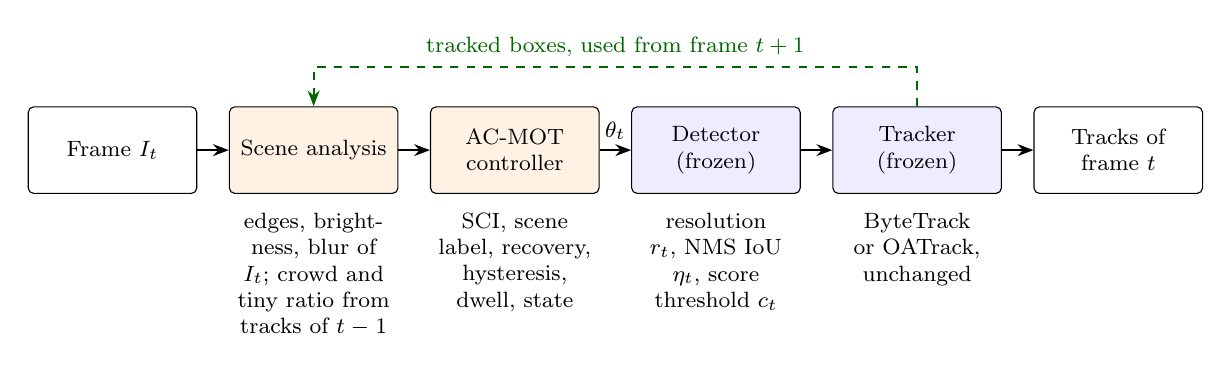
\begin{tikzpicture}[
  font=\footnotesize,
  node distance=4mm,
  stage/.style={draw, rounded corners=2pt, align=center, text width=20mm,
                minimum height=11mm, inner sep=2pt},
  ctrl/.style={stage, fill=orange!10},
  host/.style={stage, fill=blue!7},
  note/.style={align=center, text width=22.5mm, font=\footnotesize, inner sep=1pt},
  arr/.style={-{Stealth[length=2mm]}, thick},
  fb/.style={-{Stealth[length=2mm]}, thick, dashed, green!40!black}]
\node[stage] (frame) {Frame $I_t$};
\node[ctrl, right=of frame] (scene) {Scene analysis};
\node[ctrl, right=of scene] (ctrl) {AC-MOT\\controller};
\node[host, right=of ctrl] (det) {Detector\\(frozen)};
\node[host, right=of det] (trk) {Tracker\\(frozen)};
\node[stage, right=of trk] (out) {Tracks of\\frame $t$};
\draw[arr] (frame) -- (scene);
\draw[arr] (scene) -- (ctrl);
\draw[arr] (ctrl) -- node[above, font=\footnotesize] {$\theta_t$} (det);
\draw[arr] (det) -- (trk);
\draw[arr] (trk) -- (out);
\node[note, below=2mm of scene] {edges, brightness, blur of $I_t$; crowd and tiny ratio from tracks of $t-1$};
\node[note, below=2mm of ctrl] {SCI, scene label, recovery, hysteresis, dwell, state};
\node[note, below=2mm of det] {resolution $r_t$, NMS IoU $\eta_t$, score threshold $c_t$};
\node[note, below=2mm of trk] {ByteTrack or OATrack, unchanged};
\draw[fb] (trk.north) -- ++(0,5mm) -| node[pos=0.25, above, font=\footnotesize]
  {tracked boxes, used from frame $t+1$} (scene.north);
\end{tikzpicture}

\caption{AC-MOT in a tracking-by-detection pipeline. Scene analysis and the
controller choose the operating point $\theta_t=(c_t,\eta_t,r_t)$ before the
detector runs. The frozen detector and tracker are not modified. Tracked boxes
of frame $t$ feed the scene analysis of later frames (dashed arrow).}
\label{fig:pipeline}
\end{figure*}

\subsection{Scene analysis}
Scene analysis runs on frame 1 and then every ten frames ($t=1$ or
$t \bmod 10 = 1$); analysis step $j$ denotes the $j$-th such frame. Two kinds
of cues are computed.

\emph{Image cues of the current frame.} The frame is reduced to quarter scale
and converted to gray. The edge cue $e_t$ is the fraction of Canny edge pixels
(thresholds 50 and 120), the brightness cue $\beta_t$ is the mean gray level,
and the blur cue $\nu_t$ is the variance of the Laplacian.

\emph{Box cues of earlier frames.} Let $N_j$ be the number of boxes that the
tracker reported for frame $t-1$. The crowd cue and the tiny-object ratio are
\begin{align}
C_j&=\min\!\left(\frac{N_j}{30},1\right),\label{eq:crowd}\\
T_j&=\frac{1}{N_j}\sum_{i=1}^{N_j}\mathbf{1}\!\left[a_i<32^2\right],\label{eq:tiny}
\end{align}
where $a_i$ is the area of box $i$ in image pixels and $T_j=0$ when $N_j=0$.

\subsection{Crowd-selected SCI and scene label}
The SCI of the frozen controller is the mean of the most recent crowd values,
\begin{equation}
S_j=\frac{1}{|H_j|}\sum_{k\in H_j} C_k,
\label{eq:sci}
\end{equation}
where $H_j$ holds the last seven analysis steps (fewer at the start of a
sequence). The weighted SCI uses the crowd cue alone because the cue audit of
Sect.~\ref{sec:modern} selected the subset \{crowd\}. The other cues are still
computed and still act on the state, as guard and auxiliary cues. They define
a scene label $\ell_j$:
\emph{night} if $\beta_t<80$; otherwise \emph{blur} if $\nu_t<180$; otherwise
\emph{tiny} if $T_j>0.50$; otherwise \emph{crowded} if $C_j>0.65$ or
$e_t>0.13$; otherwise \emph{clear}. The tiny ratio also guards the HIGH state
directly, as shown next.

\subsection{Three-state controller}
The controller has three states, LOW, MEDIUM, and HIGH. The names describe
scene difficulty. They are not a ranking of input resolution: in the frozen
action map the HIGH state uses the smallest input (Table~\ref{tab:actions}).
At each analysis step the state is updated in the order of
Fig.~\ref{fig:state} and Algorithm~\ref{alg:controller}.

\emph{Target.} The target is HIGH if $S_j>\tau_h$ or $T_j>0.50$, MEDIUM if
$S_j>\tau_m$ or $\ell_j\in\{\text{crowded},\text{tiny}\}$, and LOW otherwise,
with the frozen thresholds $\tau_m$ and $\tau_h$ of Table~\ref{tab:constants}.

\emph{Recovery probe.} The controller keeps a decaying peak $P_j$ of the box
count. When $P_{j-1}\geq5$ and $N_j<0.40\,P_{j-1}$, a drop age $d_j$ is
increased; otherwise $d_j=0$. The peak is then updated as
$P_j=\max(N_j,\lfloor 0.8\,P_{j-1}\rfloor)$. While $1\leq d_j\leq3$, the
target is set to HIGH. This gives a short, bounded response when the number
of tracked objects collapses.

\emph{Hysteresis.} Only downward moves are held. In the HIGH state, a lower
target is ignored while $S_j>0.50$ or $T_j>0.40$. In the MEDIUM state, a lower
target is ignored while $S_j>0.25$.

\emph{Dwell.} The state cannot change within 30 frames of the last change.
The controller starts in LOW, and the state is held between analysis frames.

\begin{figure}[t]
\centering
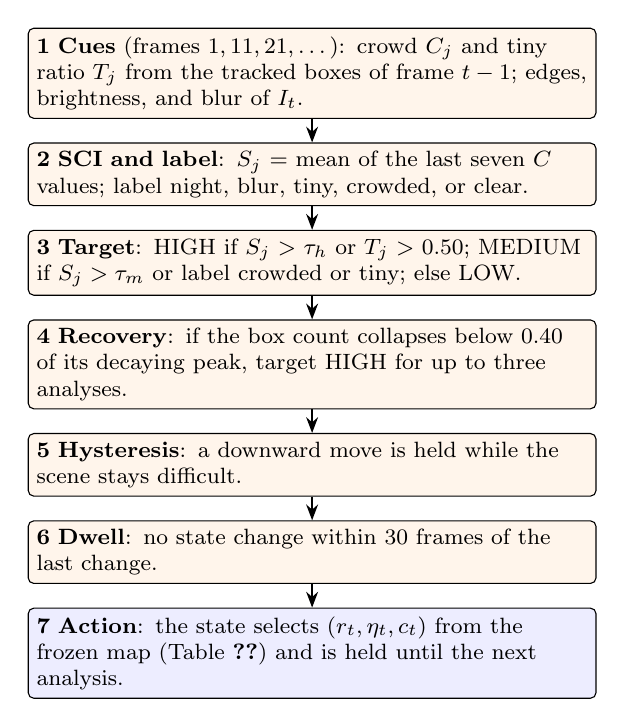
\begin{tikzpicture}[
  font=\footnotesize,
  node distance=3mm,
  blk/.style={draw, rounded corners=2pt, align=left, text width=70mm,
               inner sep=3pt, fill=orange!8},
  arr/.style={-{Stealth[length=2mm]}, thick}]
\node[blk] (cues) {\textbf{1 Cues} (frames $1, 11, 21, \dots$): crowd $C_j$ and
  tiny ratio $T_j$ from the tracked boxes of frame $t-1$; edges, brightness,
  and blur of $I_t$.};
\node[blk, below=of cues] (sci) {\textbf{2 SCI and label}: $S_j$ = mean of the
  last seven $C$ values; label night, blur, tiny, crowded, or clear.};
\node[blk, below=of sci] (target) {\textbf{3 Target}: HIGH if $S_j>\tau_h$ or
  $T_j>0.50$; MEDIUM if $S_j>\tau_m$ or label crowded or tiny; else LOW.};
\node[blk, below=of target] (probe) {\textbf{4 Recovery}: if the box count
  collapses below 0.40 of its decaying peak, target HIGH for up to three
  analyses.};
\node[blk, below=of probe] (hold) {\textbf{5 Hysteresis}: a downward move is
  held while the scene stays difficult.};
\node[blk, below=of hold] (dwell) {\textbf{6 Dwell}: no state change within 30
  frames of the last change.};
\node[blk, below=of dwell, fill=blue!7] (act) {\textbf{7 Action}: the state
  selects $(r_t, \eta_t, c_t)$ from the frozen map (Table~\ref{tab:actions}) and
  is held until the next analysis.};
\foreach \a/\b in {cues/sci, sci/target, target/probe, probe/hold, hold/dwell, dwell/act}
  \draw[arr] (\a) -- (\b);
\end{tikzpicture}

\caption{Update order of the frozen three-state controller at an analysis
frame.}
\label{fig:state}
\end{figure}

\begin{algorithm}[t]
\caption{Frozen AC-MOT controller for one sequence}\label{alg:controller}
\begin{algorithmic}[1]
\State $q\gets$ LOW; $H\gets\emptyset$; $P,d\gets0$; $t_c\gets1$
\For{each frame $t=1,2,\dots$}
  \If{$t=1$ \textbf{or} $t \bmod 10=1$}
    \State $e_t,\beta_t,\nu_t\gets$ statistics of $I_t$
    \State $N,C,T\gets$ box cues of frame $t-1$
    \State add $C$ to $H$ (keep 7); $S\gets\mathrm{mean}(H)$
    \State $\ell\gets$ scene label; $g\gets$ target from $S,T,\ell$
    \If{$P\geq5$ \textbf{and} $N<0.4P$} $d\gets d+1$
    \Else{} $d\gets0$
    \EndIf
    \State $P\gets\max(N,\lfloor0.8P\rfloor)$
    \If{$1\leq d\leq3$} $g\gets$ HIGH
    \EndIf
    \State apply the downward holds of Table~\ref{tab:constants}
    \If{$t-t_c\geq30$ \textbf{and} $g\neq q$}
      \State $q\gets g$; $t_c\gets t$
    \EndIf
  \EndIf
  \State $(r_t,\eta_t,c_t)\gets$ action of state $q$
  \State detect with $(r_t,\eta_t)$; drop scores $<c_t$
  \State update the tracker; store its boxes
\EndFor
\end{algorithmic}
\end{algorithm}

\subsection{Frozen constants and action map}
Table~\ref{tab:constants} lists the frozen constants and
Table~\ref{tab:actions} the frozen action map. LOW uses the largest input
(1536 pixels) with loose NMS and a low score threshold. MEDIUM uses 1280
pixels with tight NMS and a score threshold of 0.40. HIGH uses 1088 pixels
with NMS 0.60 and a score threshold of 0.40. The actions were selected on
calibration data together with $\tau_m$ and $\tau_h$
(Sect.~\ref{sec:modern}). The score threshold $c_t$ is applied on the detector
side before the tracker. It is separate from any confidence gate inside the
tracker, such as the fixed tracker-side gate of OATrack.

\subsection{How the constants were set}\label{sec:constants}
The constants were set with parameter sweeps and experiments, not by hand.
The analysis stride and the SCI window come from a temporal sweep on the
VisDrone validation sequences. It tested 25 combinations, with windows of 1,
3, 5, 7, and 9 analyses and strides of 1, 5, 10, 15, and 20 frames. Among the
settings that met the speed and identity constraints (at least 25 FPS and at
most 271 IDS), a window of 7 and a stride of 10 gave the highest MOTA.
Operating-point sweeps on the same data covered input resolutions from 512 to
960 pixels, confidence thresholds from 0.05 to 0.50, and NMS thresholds from
0.30 to 0.80, and defined the supported values of the first optimized
profiles (Sect.~\ref{sec:development}). The cue subset, the thresholds $\tau_m$
and $\tau_h$, and the action map were selected by cross-validated search on
separate calibration sequences (Sect.~\ref{sec:modern}). The remaining
constants of Table~\ref{tab:constants} were kept fixed in all development
stages.

\begin{table}[t]
\caption{Frozen constants of the AC-MOT scene layer.}
\label{tab:constants}
\centering\footnotesize
\begin{tabular}{@{}p{43mm}l@{}}
\toprule
Constant & Value\\
\midrule
Analysis stride (frames) & 10\\
SCI window (analysis steps) & 7\\
Crowd normalizer (boxes) & 30\\
Tiny-object area (pixels) & $32\times32$\\
MEDIUM threshold $\tau_m$ & 0.29747709701135766\\
HIGH threshold $\tau_h$ & 0.5114928923560124\\
Tiny guard for HIGH & 0.50\\
Label thresholds: brightness, blur & 80, 180\\
Label thresholds: crowd, edges & 0.65, 0.13\\
Recovery: min.\ peak, drop ratio, peak decay, steps & 5, 0.40, 0.80, 3\\
Holds: HIGH ($S$, $T$), MEDIUM ($S$) & (0.50, 0.40), 0.25\\
Dwell (frames) & 30\\
Initial state & LOW\\
\bottomrule
\end{tabular}
\end{table}

\begin{table}[t]
\caption{Frozen action map. State names describe scene difficulty, not a
resolution rank.}
\label{tab:actions}
\centering\footnotesize
\begin{tabular}{@{}lrrr@{}}
\toprule
State & Resolution $r$ & NMS IoU $\eta$ & Score threshold $c$\\
\midrule
LOW & 1536 & 0.70 & 0.10\\
MEDIUM & 1280 & 0.45 & 0.40\\
HIGH & 1088 & 0.60 & 0.40\\
\bottomrule
\end{tabular}
\end{table}

\section{How the Final Controller Was Developed}\label{sec:development}

The controller was developed in four steps: a quality-oriented profile, an
identity-aware profile, transfer and cross-pipeline studies, and a modern
stage that produced the frozen controller. Each step is compared with the
baseline it was built on. The historical steps used other detectors and
evaluation protocols than the modern stage, so their numbers are reported in
their own tables and are not pooled with the modern results.

\subsection{Quality-oriented profile}\label{sec:quality}

\emph{Baseline.} The reference pipeline is the pretrained YOLOv8n detector
\cite{jocher2023yolov8} followed by ByteTrack \cite{zhang2022bytetrack}, both at
their default settings: confidence threshold 0.25, NMS IoU threshold 0.45,
input size 640 pixels, and the default ByteTrack parameters (high threshold
0.25, low threshold 0.10, new-track threshold 0.25, buffer 30 frames, match
threshold 0.80). It runs with one fixed operating point for the whole video.

\emph{Method.} The first optimization-derived profile kept the same detector,
used a tuned ByteTrack profile, and searched only on the VisDrone2019-MOT
validation split. Five cues were used: crowd count, the fraction of earlier
boxes below $32\times32$ pixels, edge density, low brightness, and low
Laplacian variance. Each cue was normalized with validation statistics, and
the index was their weighted sum
\begin{equation}
S_j=\sum_{k\in\{c,t,e,n,b\}}w_k\,x_{k,j},
\label{eq:hist-sci}
\end{equation}
with $w_k\geq0$ and $\sum_k w_k=1$, averaged over seven analyses taken every
ten frames. Confidence and NMS were interpolated linearly between the values
at $S=0$ and $S=1$, and two sorted thresholds selected one of three
resolutions (512, 928, 960 pixels).

An Optuna TPE study \cite{akiba2019optuna} jointly searched the five weights,
the confidence and NMS end points, and the two thresholds. The resolution
levels, the supported confidence values $\{0.25,\dots,0.45\}$, the supported
NMS values from 0.30 to 0.70, and the temporal settings were fixed beforehand
by validation sweeps (Sect.~\ref{sec:constants}). The selection rule kept
trials with at least 25 FPS and at most 271 IDS (a reference value from
earlier validation runs) and then took the highest MOTA, with lower IDS, HOTA,
IDF1, and FPS as tie-breaks. The frozen profile (archived as Trial~24) has
$w_c=0.1294928$, $w_t=0.2217477$, $w_e=0.4337134$, $w_n=0.0535577$,
$w_b=0.1614885$, confidence end points $(0.30,0.40)$, NMS end points
$(0.35,0.35)$, and thresholds $(0.1353494, 0.2872868)$. On validation it
reached MOTA 23.038, HOTA 36.110, IDF1 40.758, and IDS 270 at 37.169 FPS.

\emph{Comparison.} Table~\ref{tab:quality} compares the profile with the
baseline on the historical VisDrone test-dev split, with paired bootstrap
intervals (5000 resamples, seed 42). HOTA rises by 5.4051 points, MOTA by
7.2195 points, and IDF1 by 8.8220 points, and throughput rises from 36.528 to
38.985 FPS.

\begin{table}[t]
\caption{Quality-oriented profile versus its baseline (YOLOv8n with ByteTrack
at default settings) on VisDrone test-dev, historical protocol. Gain: paired
bootstrap difference with 95\% interval; for IDS it is the reduction.}
\label{tab:quality}
\centering\footnotesize
\setlength{\tabcolsep}{4pt}
\begin{tabular}{@{}lrrl@{}}
\toprule
Metric & Baseline & Quality & Gain [95\% CI]\\
\midrule
HOTA & 28.430 & 33.835 & $+5.4051$ $[4.1273, 6.9022]$\\
MOTA & 19.729 & 26.948 & $+7.2195$ $[5.4362, 9.2934]$\\
IDF1 & 32.724 & 41.546 & $+8.8220$ $[6.9005, 11.0537]$\\
IDS & 1235 & 1184 & $51$ $[-114, 219]$\\
FPS & 36.528 & 38.985 & --\\
\bottomrule
\end{tabular}
\end{table}

\subsection{Identity-aware Pareto profile}\label{sec:identity}

\emph{Baseline.} The baseline is the same YOLOv8n and ByteTrack pipeline at
default settings (Sect.~\ref{sec:quality}).

\emph{Method.} Quality is not the only deployment goal; identity stability and
compute can move in a different direction from MOTA. The second study kept
the same cues, operating levels, temporal settings, and validation data, but
changed the question. It maximized MOTA and minimized IDS subject only to
$\mathrm{FPS}\geq25$, without the IDS gate. A seeded TPE sampler ran 49
completed trials. A trial dominated another when it had no lower MOTA and no
higher IDS, with at least one strict improvement, and the feasible Pareto
front was built from these relations \cite{deb2002nsga2}. The balanced
candidate maximized an equal-weight score of normalized MOTA and normalized IDS
reduction, with HOTA, IDF1, FPS, and trial index as tie-breaks.

The selected profile (archived as Trial~22) has weights $w_c=0.1646453$,
$w_t=0.1746265$, $w_e=0.5076113$, $w_n=0.1206956$, $w_b=0.0324213$,
confidence end points $(0.40,0.40)$, NMS end points $(0.60,0.35)$, and
thresholds $(0.2927136, 0.6661672)$. On validation it reached MOTA 19.330,
HOTA 31.651, IDF1 34.226, and IDS 168 at 51.406 FPS.

\emph{Comparison.} Table~\ref{tab:identity} compares the profile with the
baseline on test-dev. It removes 316 identity switches and raises throughput
from 36.528 to 46.024 FPS, while HOTA, MOTA, and IDF1 also rise. Against the
quality-oriented profile it has 265 fewer IDS $[82, 502]$ and $-2.617$ HOTA
$[-4.004, -1.694]$. The two profiles therefore answer different questions: one
favors overall quality and the other favors identity stability and speed.

\begin{table}[t]
\caption{Identity-aware profile versus its baseline (YOLOv8n with ByteTrack at
default settings) on VisDrone test-dev, historical protocol. Gain: paired
bootstrap difference with 95\% interval; for IDS it is the reduction.}
\label{tab:identity}
\centering\footnotesize
\setlength{\tabcolsep}{4pt}
\begin{tabular}{@{}lrrl@{}}
\toprule
Metric & Baseline & Identity & Gain [95\% CI]\\
\midrule
HOTA & 28.430 & 31.218 & $+2.788$ $[0.747, 4.660]$\\
MOTA & 19.729 & 23.792 & $+4.063$ $[0.952, 6.886]$\\
IDF1 & 32.724 & 37.870 & $+5.146$ $[2.028, 8.080]$\\
IDS & 1235 & 919 & $316$ $[175, 470]$\\
FPS & 36.528 & 46.024 & --\\
\bottomrule
\end{tabular}
\end{table}

\subsection{Transfer and cross-pipeline studies}\label{sec:transfer}

\emph{UAVDT.} The baseline is again YOLOv8n with ByteTrack at default settings
(Sect.~\ref{sec:quality}). Both frozen profiles were applied to UAVDT
\cite{du2018uavdt} without retuning (Table~\ref{tab:hist-uavdt}). The
quality-oriented profile raised HOTA by 4.305 points $[2.740, 5.709]$ and the
identity-aware profile by 2.845 points $[1.238, 4.348]$; their IDS reductions
are 237 $[104, 377]$ and 250 $[110, 404]$.

\begin{table}[t]
\caption{Historical UAVDT transfer without retuning. Baseline: YOLOv8n with
ByteTrack at default settings.}
\label{tab:hist-uavdt}
\centering\footnotesize
\setlength{\tabcolsep}{4pt}
\begin{tabular}{@{}lrrr@{}}
\toprule
Metric & Baseline & Quality & Identity\\
\midrule
HOTA & 24.085 & 28.390 & 26.930\\
MOTA & 13.841 & 17.399 & 16.118\\
IDF1 & 27.887 & 34.453 & 32.014\\
IDS & 558 & 321 & 308\\
FPS & 65.015 & 58.353 & 61.462\\
\bottomrule
\end{tabular}
\end{table}

\emph{U2MOT on VisDrone.} The baseline is the published U2MOT tracker
\cite{liu2023u2mot} with its released YOLOX-X detector \cite{ge2021yolox}, run
at its own static setting. Seven VisDrone validation sequences served for
development and 17 test-dev sequences for evaluation. The cue weights and
transforms of the quality-oriented profile were kept, the tracker was not
modified, and the action boundaries were set to the 33rd and 67th percentiles
of the index on the U2MOT validation run, without using ground truth.
Table~\ref{tab:u2mot} gives the comparison: the controlled pipeline has 87
fewer IDS and 1230 fewer FP.

\begin{table}[t]
\caption{Cross-pipeline study on VisDrone test-dev. Baseline: U2MOT with its
YOLOX-X detector at its static setting.}
\label{tab:u2mot}
\centering\footnotesize
\setlength{\tabcolsep}{4pt}
\begin{tabular}{@{}lrr@{}}
\toprule
Metric & U2MOT baseline & With controller\\
\midrule
MOTA & 53.873 & 53.767\\
IDF1 & 69.775 & 69.849\\
IDS & 1239 & 1152\\
FP & 41385 & 40155\\
FN & 63241 & 64801\\
\bottomrule
\end{tabular}
\end{table}

\emph{SparseTrack on MOT17.} The baseline is the published SparseTrack tracker
\cite{liu2025sparsetrack} with a fixed NMS IoU threshold of 0.75, on the seven
MOT17 \texttt{val\_half} sequences (2652 frames) \cite{milan2020motchallenge}.
A minimal edge-driven rule switched only the NMS threshold, between 0.70 and
0.80; its threshold came from a leave-one-sequence-out study on the same
sequences. Table~\ref{tab:sparsetrack} gives the comparison: the adaptive rule
reduces IDS from 136 to 123, with MOTA $+0.0371$ points $[-0.041, +0.182]$.

\begin{table}[t]
\caption{Cross-pipeline study on MOT17 \texttt{val\_half}. Baseline:
SparseTrack with a fixed NMS IoU threshold of 0.75.}
\label{tab:sparsetrack}
\centering\footnotesize
\setlength{\tabcolsep}{4pt}
\begin{tabular}{@{}lrr@{}}
\toprule
Metric & SparseTrack baseline & With adaptive NMS\\
\midrule
MOTA & 76.8881 & 76.9252\\
IDF1 & 81.4943 & 81.5299\\
IDS & 136 & 123\\
\bottomrule
\end{tabular}
\end{table}

Together these studies show that the preferred profile depends on the
objective (quality or identity) and on the tracker host. This motivated a
modern stage with a stronger detector, explicit calibration data, and two
tracker hosts.

\subsection{Modern development of the frozen controller}\label{sec:modern}

\emph{Baseline.} The modern baseline is the YOLO11m detector
\cite{jocher2024yolo11}, in the public VisDrone checkpoint described in
Sect.~\ref{sec:setup}, run at a fixed operating point of 1536 pixels and NMS
IoU 0.70 with no extra score threshold. It feeds ByteTrack
\cite{zhang2022bytetrack} during development and both ByteTrack and OATrack
\cite{qi2026oatrack} in the final evaluation. A large fixed input is a common
choice for small aerial objects when no adaptation is used.

\emph{Data and protocol.} Eight sequences of the VisDrone2019-MOT training split
(3282 frames) were declared as calibration data. They are disjoint from the
seven evaluation sequences. All development used four folds, each holding out
two calibration sequences, and reported the cross-validated (CV) mean change
in HOTA against the baseline. Detector outputs were cached for every
resolution and NMS value; a score threshold applied to the cache was checked
to reproduce direct inference exactly. Table~\ref{tab:devrecord} summarizes
the development steps.

\emph{Cue audit.} Stages 1 and 2 searched the state-to-resolution and
state-to-NMS maps on exhaustive grids. Stage 3A searched all 31 non-empty
subsets of the five cues and selected \{crowd\}, which defines the
crowd-selected SCI of Eq.~\eqref{eq:sci}. The other cues were kept as guard and
auxiliary cues of the state logic (Sect.~\ref{sec:method}).

\emph{Score threshold.} At 1088 pixels and NMS 0.45, a fixed score threshold
of 0.40 raised pooled calibration HOTA by $+0.881$ over 0.01 and improved
seven of the eight sequences. The score threshold was therefore added as the
third action dimension.

\emph{Final joint search.} The final search used 60 TPE trials (seed 43). It
searched $\tau_m\in[0.10,0.50]$, $\tau_h\in[\tau_m+0.05,\min(\tau_m+0.40,0.90)]$,
and for each state a resolution in $\{1088,1280,1536\}$, an NMS value in
$\{0.45,0.60,0.70\}$, and a score threshold in $\{0.10,0.25,0.40\}$. The
objective was the CV mean change in HOTA against the baseline, with ByteTrack
as host. Eligible candidates had to realize at least two distinct actions,
each on at least 10\% of calibration frames, and switch within sequences. The
frozen policy is the eligible candidate whose three states use three
different actions (Table~\ref{tab:actions}). On calibration data it used LOW,
MEDIUM, and HIGH on 7.6\%, 10.1\%, and 82.3\% of frames, with 0.607 state
changes per 100 frames on average.

\emph{Comparison.} Table~\ref{tab:folds} compares the frozen policy with the
baseline on each calibration fold. All four folds are positive, with a CV
mean of $+2.447$ HOTA. After these steps the thresholds, cue subset, and
action map were frozen. The final comparison on the evaluation sequences is
given in Sect.~\ref{sec:results}.

\begin{table}[t]
\caption{Main modern development steps on the eight calibration sequences
(ByteTrack host). The score-threshold gain is pooled HOTA; the joint-search
result is the mean over four folds.}
\label{tab:devrecord}
\centering\footnotesize
\setlength{\tabcolsep}{3pt}
\begin{tabular}{@{}lll@{}}
\toprule
Step & Search & Result\\
\midrule
Cue subset & 31 subsets & \{crowd\}\\
Score threshold & 4 values & 0.40; $+0.881$ HOTA\\
Joint search & 60 TPE trials & CV mean $+2.447$\\
\bottomrule
\end{tabular}
\end{table}

\begin{table}[t]
\caption{Frozen policy versus the modern baseline (YOLO11m at 1536 pixels and
NMS 0.70, ByteTrack) on the four calibration folds: change in HOTA.}
\label{tab:folds}
\centering\footnotesize
\begin{tabular}{@{}lrrrrr@{}}
\toprule
 & Fold 1 & Fold 2 & Fold 3 & Fold 4 & Mean\\
\midrule
$\Delta$HOTA & $+0.592$ & $+4.164$ & $+2.029$ & $+3.004$ & $+2.447$\\
\bottomrule
\end{tabular}
\end{table}

\section{Experimental Setup}\label{sec:setup}

\subsection{Detector and tracker hosts}
All modern experiments use one frozen public YOLO11m detector
\cite{jocher2024yolo11}, the
Hugging Face checkpoint \texttt{dronefreak/\allowbreak visdrone-\allowbreak yolo11m}. It was
trained on VisDrone2019-DET at 640 pixels (SHA256 \checkpointsha). It runs in half precision. Detections of the
classes pedestrian, car, van, truck, and bus are passed on.

Two tracker hosts are used and kept unchanged. ByteTrack uses the Ultralytics
implementation with high threshold 0.25, low threshold 0.10, new-track
threshold 0.25, buffer 30 frames, and match threshold 0.80. OATrack is a
re-implementation of the published method \cite{qi2026oatrack} in its main
configuration, with a tracker-side confidence gate of 0.40. This gate belongs
to the tracker and is never changed by AC-MOT.

\subsection{Systems}
The baseline runs the detector at the fixed operating point of 1536 pixels and
NMS IoU 0.70, with no score threshold above the cache floor of 0.01. AC-MOT
runs the frozen controller of Sect.~\ref{sec:method} on the same detector. For
each host, the baseline and AC-MOT differ only in the detector operating
point.

\subsection{Data}
The VisDrone evaluation uses seven sequences of the VisDrone2019-MOT
validation split. They contain 71,830 ground-truth boxes. The cue subset,
thresholds, and action map of the frozen controller were selected on the
separate calibration sequences only (Sect.~\ref{sec:modern}). The UAVDT transfer uses 20 test
sequences with 16,592 frames. The frozen controller, thresholds, and action
map are applied without any change. Detector outputs for UAVDT were produced
at the three frozen operating points, giving 49,776 detector forward passes.

\subsection{Metrics and evaluation}
VisDrone results are scored with a Python port of the VisDrone2019-MOT
Task~4b evaluation. Ignored regions are removed, the five classes above are
evaluated separately, CLEAR-MOT and identity measures use IoU 0.5, and counts
are summed over classes and sequences. HOTA is added with the same class-aware
scheme using TrackEval. UAVDT is scored with one vehicle class. We report
HOTA \cite{luiten2021hota}, MOTA, IDF1, IDS, FP, FN, precision, and recall.

Uncertainty on VisDrone is estimated with a paired bootstrap at the sequence
level \cite{efron1993bootstrap}. Each of 5000 resamples (seed 42) draws seven
sequences with replacement. The same draw is used for both systems, the pooled
metrics are recomputed, and their difference is recorded. The 95\% interval
is the 2.5--97.5 percentile range. UAVDT is a single frozen run per host.

Latency is measured on one Tesla T4 GPU over the first 200 frames of sequence
\texttt{uav0000086\_00000\_v}, excluding five warm-up frames. For every
frame, the time spent in the controller (image statistics, scene analysis, and
state update) is recorded separately from the detector and tracker time.

\section{Results}\label{sec:results}

\subsection{Frozen VisDrone evaluation}
Table~\ref{tab:visdrone} lists the aggregate results on the seven VisDrone
sequences, and Fig.~\ref{fig:visdrone} shows HOTA, MOTA, and IDF1.

\begin{table}[t]
\caption{Frozen VisDrone evaluation on seven VisDrone2019-MOT sequences
(71,830 ground-truth boxes). Baseline: fixed operating point (1536, 0.70).}
\label{tab:visdrone}
\centering\footnotesize
\setlength{\tabcolsep}{4pt}
\begin{tabular}{@{}lrrrr@{}}
\toprule
 & \multicolumn{2}{c}{ByteTrack} & \multicolumn{2}{c}{OATrack}\\
\cmidrule(lr){2-3}\cmidrule(l){4-5}
Metric & Baseline & AC-MOT & Baseline & AC-MOT\\
\midrule
HOTA & 41.586 & 44.523 & 46.770 & 48.095\\
MOTA & 9.876 & 27.871 & 28.165 & 34.483\\
IDF1 & 48.569 & 53.929 & 57.107 & 59.364\\
IDS & 1341 & 1016 & 773 & 604\\
FP & 39274 & 24892 & 25394 & 21400\\
FN & 24121 & 25902 & 25432 & 25057\\
Precision & 54.849 & 64.852 & 64.628 & 68.609\\
Recall & 66.419 & 63.940 & 64.594 & 65.116\\
\bottomrule
\end{tabular}
\end{table}

\emph{ByteTrack host.} AC-MOT changes HOTA from 41.586 to 44.523, MOTA from
9.876 to 27.871, and IDF1 from 48.569 to 53.929. IDS fall from 1341 to 1016
and FP from 39274 to 24892, while FN rise from 24121 to 25902. Precision rises
from 54.849 to 64.852 and recall falls from 66.419 to 63.940. The detector
output becomes more selective: clutter and identity-confusing boxes are
removed at a small cost in recall.

\emph{OATrack host.} AC-MOT changes HOTA from 46.770 to 48.095, MOTA from
28.165 to 34.483, and IDF1 from 57.107 to 59.364. IDS fall from 773 to 604, FP
from 25394 to 21400, and FN from 25432 to 25057. Precision rises from 64.628 to
68.609 and recall from 64.594 to 65.116. OATrack starts from a stronger
baseline.

\begin{figure}[t]
\centering
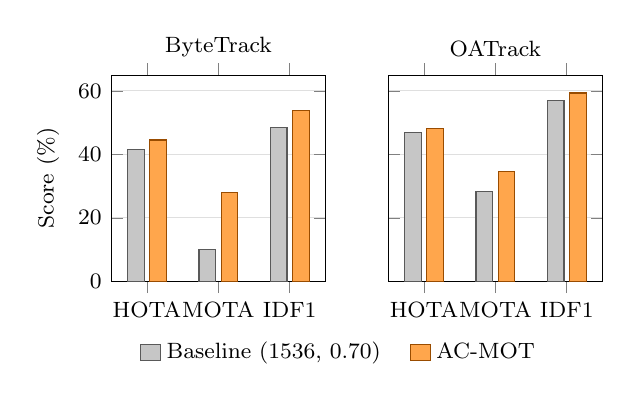
\begin{tikzpicture}
\begin{groupplot}[
  group style={group size=2 by 1, horizontal sep=8mm},
  width=43mm, height=42mm,
  ybar, /pgf/bar width=6pt, ymin=0, ymax=65,
  symbolic x coords={HOTA,MOTA,IDF1}, xtick=data,
  enlarge x limits=0.25,
  ymajorgrids, grid style={gray!25},
  tick label style={font=\footnotesize},
  title style={font=\footnotesize, yshift=-1mm},
  ylabel style={font=\footnotesize},
  legend style={font=\footnotesize, draw=none, legend columns=2,
                at={(1.07,-0.24)}, anchor=north, /tikz/every even column/.append style={column sep=3mm}},
  legend image code/.code={\draw[#1] (0cm,-0.1cm) rectangle (0.25cm,0.1cm);}]
\nextgroupplot[title={ByteTrack}, ylabel={Score (\%)}]
\addplot[fill=gray!45, draw=gray!70!black] coordinates {(HOTA,41.586) (MOTA,9.876) (IDF1,48.569)};
\addplot[fill=orange!70, draw=orange!60!black] coordinates {(HOTA,44.523) (MOTA,27.871) (IDF1,53.929)};
\legend{{Baseline (1536, 0.70)}, {AC-MOT}}
\nextgroupplot[title={OATrack}, yticklabels={}]
\addplot[fill=gray!45, draw=gray!70!black] coordinates {(HOTA,46.770) (MOTA,28.165) (IDF1,57.107)};
\addplot[fill=orange!70, draw=orange!60!black] coordinates {(HOTA,48.095) (MOTA,34.483) (IDF1,59.364)};
\end{groupplot}
\end{tikzpicture}

\caption{HOTA, MOTA, and IDF1 on the seven VisDrone sequences for both
tracker hosts (values in Table~\ref{tab:visdrone}).}
\label{fig:visdrone}
\end{figure}

\subsection{Paired bootstrap}
\begin{table}[t]
\caption{Paired sequence-level bootstrap on VisDrone: AC-MOT minus baseline,
5000 resamples, seed 42. HOTA, MOTA, IDF1, precision, and recall in points;
IDS, FP, and FN in counts.}
\label{tab:bootstrap}
\centering\footnotesize
\setlength{\tabcolsep}{4pt}
\begin{tabular}{@{}llrr@{}}
\toprule
Host & Metric & Difference & 95\% interval\\
\midrule
ByteTrack & HOTA & $+2.937$ & $[+2.356, +3.375]$\\
 & MOTA & $+17.995$ & $[+13.541, +23.282]$\\
 & IDF1 & $+5.360$ & $[+4.490, +6.178]$\\
 & IDS & $-325$ & $[-498, -164]$\\
 & FP & $-14382$ & $[-19176, -9620]$\\
 & FN & $+1781$ & $[+288, +3594.075]$\\
 & Precision & $+10.003$ & $[+8.712, +11.895]$\\
 & Recall & $-2.479$ & $[-4.507, -0.469]$\\
\midrule
OATrack & HOTA & $+1.325$ & $[+0.200, +2.264]$\\
 & MOTA & $+6.318$ & $[+4.741, +7.879]$\\
 & IDF1 & $+2.258$ & $[+0.548, +3.474]$\\
 & IDS & $-169$ & $[-292, -42]$\\
 & FP & $-3994$ & $[-6190, -2494.900]$\\
 & FN & $-375$ & $[-1462.575, +670]$\\
 & Precision & $+3.981$ & $[+2.957, +5.511]$\\
 & Recall & $+0.522$ & $[-0.869, +2.111]$\\
\bottomrule
\end{tabular}
\end{table}

Table~\ref{tab:bootstrap} gives the paired differences (AC-MOT minus baseline)
and their 95\% intervals. With ByteTrack, the intervals of HOTA, MOTA, IDF1,
precision, IDS, and FP lie entirely on the side of improvement, and FN and
recall move in the opposite direction. With OATrack, HOTA, MOTA, IDF1, and
precision rise and IDS and FP fall, all with intervals on one side of zero.

\subsection{Controller behaviour}

The controller uses all three states with both hosts. With ByteTrack, LOW,
MEDIUM, and HIGH cover 7.4\%, 30.1\%, and 62.5\% of the frames; with OATrack
they cover 7.4\%, 33.3\%, and 59.3\%. The two hosts diverge through their
different tracked boxes. State changes are rare, between 0.10 and 0.54 per 100
frames depending on the sequence, so the detector input stays stable over
long stretches of video.

\subsection{Frozen UAVDT transfer}
\begin{table}[t]
\caption{Frozen UAVDT transfer without retuning (20 sequences, 16,592 frames,
one vehicle class). Baseline: fixed operating point (1536, 0.70).}
\label{tab:uavdt}
\centering\footnotesize
\setlength{\tabcolsep}{4pt}
\begin{tabular}{@{}lrrrr@{}}
\toprule
 & \multicolumn{2}{c}{ByteTrack} & \multicolumn{2}{c}{OATrack}\\
\cmidrule(lr){2-3}\cmidrule(l){4-5}
Metric & Baseline & AC-MOT & Baseline & AC-MOT\\
\midrule
HOTA & 45.923 & 47.004 & 47.728 & 47.640\\
MOTA & $-1.573$ & 16.028 & 19.607 & 22.873\\
IDF1 & 58.400 & 61.767 & 62.101 & 62.931\\
IDS & 601 & 486 & 517 & 486\\
FP & 279616 & 212077 & 197937 & 183669\\
FN & 66050 & 73702 & 75612 & 78774\\
Precision & 49.571 & 55.751 & 57.270 & 58.800\\
Recall & 80.625 & 78.381 & 77.820 & 76.893\\
\bottomrule
\end{tabular}
\end{table}

Table~\ref{tab:uavdt} and Fig.~\ref{fig:uavdt} report the transfer to UAVDT
without retuning. With ByteTrack, HOTA changes from 45.923 to 47.004 ($+1.081$),
MOTA from $-1.573$ to 16.028 ($+17.601$), and IDF1 from 58.400 to 61.767
($+3.367$). IDS fall by 115 and FP by 67539, while FN rise by 7652. With
OATrack, MOTA changes from 19.607 to 22.873 ($+3.267$), IDF1 from 62.101 to
62.931 ($+0.831$), IDS fall by 31, and FP fall by 14268. With both hosts the
transfer gives fewer FP and IDS and higher precision, with slightly lower
recall, the same pattern as with ByteTrack on VisDrone.

\begin{figure}[t]
\centering
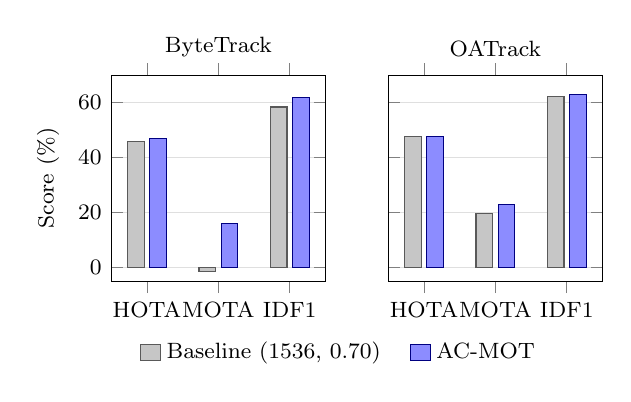
\begin{tikzpicture}
\begin{groupplot}[
  group style={group size=2 by 1, horizontal sep=8mm},
  width=43mm, height=42mm,
  ybar, /pgf/bar width=6pt, ymin=-5, ymax=70,
  symbolic x coords={HOTA,MOTA,IDF1}, xtick=data,
  enlarge x limits=0.25,
  ymajorgrids, grid style={gray!25},
  tick label style={font=\footnotesize},
  title style={font=\footnotesize, yshift=-1mm},
  ylabel style={font=\footnotesize},
  legend style={font=\footnotesize, draw=none, legend columns=2,
                at={(1.07,-0.24)}, anchor=north, /tikz/every even column/.append style={column sep=3mm}},
  legend image code/.code={\draw[#1] (0cm,-0.1cm) rectangle (0.25cm,0.1cm);}]
\nextgroupplot[title={ByteTrack}, ylabel={Score (\%)}]
\addplot[fill=gray!45, draw=gray!70!black] coordinates {(HOTA,45.923) (MOTA,-1.573) (IDF1,58.400)};
\addplot[fill=blue!45, draw=blue!50!black] coordinates {(HOTA,47.004) (MOTA,16.028) (IDF1,61.767)};
\legend{{Baseline (1536, 0.70)}, {AC-MOT}}
\nextgroupplot[title={OATrack}, yticklabels={}]
\addplot[fill=gray!45, draw=gray!70!black] coordinates {(HOTA,47.728) (MOTA,19.607) (IDF1,62.101)};
\addplot[fill=blue!45, draw=blue!50!black] coordinates {(HOTA,47.640) (MOTA,22.873) (IDF1,62.931)};
\end{groupplot}
\end{tikzpicture}

\caption{HOTA, MOTA, and IDF1 of the frozen UAVDT transfer for both tracker
hosts (values in Table~\ref{tab:uavdt}).}
\label{fig:uavdt}
\end{figure}

\section{Discussion}\label{sec:discussion}

\emph{The operating point is part of the MOT system.} The same frozen detector
and the same trackers give very different MOT results at different operating
points. Moving away from the fixed 1536/0.70 point raises MOTA by 17.995 points
with ByteTrack and by 6.318 points with OATrack on VisDrone. The detector
operating point is therefore a first-order variable of aerial MOT and deserves
the same attention as the association method.

\emph{Selective observation streams.} The main effect of AC-MOT is a more
selective detection stream. FP and IDS drop sharply, precision rises, and FN
rise a little with ByteTrack. MOTA reacts most strongly because it counts FP
directly; HOTA and IDF1 rise by smaller amounts. The same pattern appears on
UAVDT, where FP fall by 67539 with ByteTrack and by 14268 with OATrack.

\emph{Tracker dependence.} ByteTrack gains more than OATrack. ByteTrack starts
from a weaker baseline and uses low-score boxes in its second association
step, so a likely reason is that removing clutter helps it directly. OATrack
already weights detections by quality inside its association, and it gains
mainly in MOTA, IDF1, IDS, and FP. Results are therefore reported per host.

\emph{Development path.} The historical profiles showed that the preferred
operating point depends on the goal: quality or identity stability and speed.
The modern stage kept a finite, readable controller with one crowd index, a few
guard cues, three states, and three actions.

\emph{Deployment.} AC-MOT needs no training and no access to detector or
tracker internals. It changes three arguments of the detector call. Its
analysis runs on a quarter-scale image every ten frames and uses boxes that
the tracker already produced. On a Tesla T4 the controller takes 4.26 ms per
frame with ByteTrack and 4.20 ms with OATrack, which is small next to detector
inference. The control layer therefore adds very little latency and is
suitable for real-time use. The same interface can host other action maps, for
example maps chosen for a latency budget, without changes to the detector or
the tracker.

\section{Conclusion}\label{sec:conclusion}

AC-MOT is a training-free control layer that uses only the current frame and
past tracker output and adapts the detector
confidence threshold, NMS IoU threshold, and input resolution online while the
detector and the tracker stay unchanged. Its frozen form uses a crowd-selected
scene complexity index, guard cues for tiny objects, illumination, blur, and
edges, a recovery probe, hysteresis, and dwell, and a three-state action map.

The controller was developed through optimization. Quality-oriented and
identity-aware profiles, together with transfer and cross-pipeline studies,
showed that the preferred operating point depends on the objective and on the
tracker host. The modern stage froze the controller after sequence-level
cross-validation on separate calibration sequences.

On seven VisDrone2019-MOT sequences, AC-MOT raised HOTA by 2.937 points with
ByteTrack and by 1.325 points with OATrack, and MOTA by 17.995 and 6.318
points, with paired bootstrap intervals for every metric. Applied to UAVDT
without retuning, it raised MOTA by 17.601 and 3.267 points. These results
support treating the detector operating point as part of the MOT system and
controlling it online.


\backmatter

\section*{Declarations}

\noindent\textbf{Funding.} This research received no external funding.

\noindent\textbf{Conflict of interest.} The authors declare no competing interests.

\noindent\textbf{Ethics approval and consent to participate.} This computational study uses public benchmark data and does not involve human participants or animals.

\noindent\textbf{Consent for publication.} Not applicable.

\noindent\textbf{Data and code availability.} The frozen controller specification, result records, evidence map, staged sections, scripts, and build package are included in the project repository. Dataset redistribution remains subject to the original benchmark licenses and access terms.

\noindent\textbf{Author contributions.} Ahmed Gouda Ismail: Conceptualization, Methodology, Software, Investigation, Data curation, Formal analysis, Visualization, Writing~--~original draft, Writing~--~review \& editing. Mohamed S. Mohamed: Supervision, Methodology, Writing~--~review \& editing. Tarek Ahmed Mahmoud: Supervision, Validation, Writing~--~review \& editing.

\noindent\textbf{Acknowledgements.} Not applicable.

\noindent\textbf{Submission exclusivity.} The manuscript is not under consideration elsewhere and has not been published previously.

\noindent\textbf{AI use in manuscript preparation.} Generative AI tools were used to assist with drafting and language editing. The authors reviewed and verified all content, numerical values, and figures and take full responsibility for the manuscript.

\bibliography{references}

\end{document}
